\subsection{Experimental}
\subsubsection{Síntesis}
Se llevará a cabo la síntesis de los compuestos \textbf{1-4} (ver \cref{sch:marcha,sch:reac-gral}) utilizando condiciones de reacción ecológicas y materiales de partida accesibles. Se optimizarán los parámetros de reacción para obtener rendimientos elevados y selectividad adecuada.

\begin{scheme}[H]
	\centering
	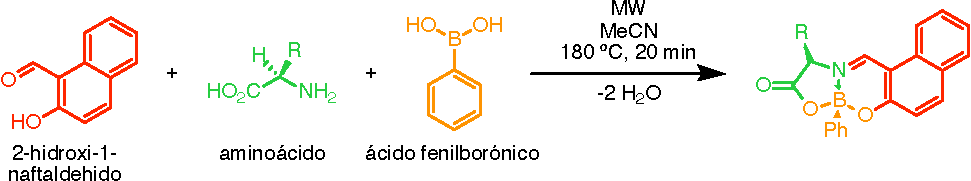
\includegraphics[width=0.85\linewidth]{./Figuras/BO-General.pdf}
	\caption[Síntesis de las BOSCHIBA por MW]{Método de síntesis para las \gls{BOSCHIBA} \textbf{1-4} por \gls{MW}.}
	\label{sch:reac-gral}
\end{scheme}

\subsubsection{Determinación de propiedades ópticas}
Se determinará el rendimiento cuántico de los compuestos \reactant{BO}, así como su contraste de fluorescencia en medios de viscosidad variable, controlado por la adición de glicerol en diferentes proporciones.

\subsubsection{Determinación de citotoxicidad}
Se determinará la citotoxicidad de los compuestos \textbf{1-4} en la línea celular de melanoma murino \emph{B16F10} (ATCC® CCL-6475™) derivado de ratón C57BL/6J.
Se incubarán las celulas por \qty{24}{\hour} a \qty{37}{\degreeCelsius} y \qty{5}{\percent} de \ch{CO2} en medio de cultivo \emph{Dulbecco's Modified Eagle Medium} (DMEM) con \qty{10}{\percent} de suero fetal bovino (FBS) y \qty{1}{\percent} de antibiótico/antimicótico (penicilina, estreptomicina y anfotericina B), según las indicaciones del fabricante.

\subsection{Ensayo de tinción celular}
Se sembrarán las células \emph{B16F10} en placas de cultivo de 96 pozos a una densidad de \qty{1.5e5}{{cell}\per{pozo}} en \qty{100}{\uL} de medio de cultivo DMEM. Después de incubarse por \qty{24}{\hour} a \qty{37}{\degreeCelsius} y \qty{5}{\percent} de \ch{CO2}, se retirará el medio de cultivo y se lavarán las células con \qty{100}{\uL} de \emph{PBS} (\qty{1}{\percent} de \ch{EDTA} y \qty{0.5}{\percent} de \ch{BSA} en \emph{PBS}). Se añadirá colorante Hoechst según las indicaciones del fabricante. Después las células serán fijadas con \qty{100}{\uL} de \ch{PFA} al \qty{4}{\percent} en \emph{PBS} por \qty{15}{\minute} a \qty{37}{\degreeCelsius} y \qty{5}{\percent} de \ch{CO2}. Se hará el ensayo por microscopía de fluorescencia.

\subsubsection{Modelado molecular}
Se realizarán cálculos \insilico{} por medio de \gls{DFT} y \gls{TDDFT} para estudiar las propiedades fotofísicas de los compuestos y comprobar los mecanismos involucrados en el efecto supresor de la luminiscencia en dichos compuestos así como estudios de topológicos sobre estos.

\paragraph{Preoptimización}
En caso de no contar con datos cristalográficos en el momento del estudio \insilico{}, se hará una búsqueda conformacional con ayuda del programa \gls{CREST} \cite{prachtAutomatedExplorationLowenergy2020} para obtener los confórmeros más estables de los compuestos.

En caso de que se cuenten con datos cristalográficos, se utilizarán las coordenadas de la estructura cristalográfica para realizar la optimización geométrica en DFT.

\paragraph{Optimización geométrica}
Se hará la optimización geométrica de los compuestos \textbf{1-4} empleando el funcional meta-GGA \scan{}\footnote{La selección de este funcional para la optimización geométrica se debe a su desempeño comparable o superior con funcionales híbridos meta-GGA como M06-2X-D3(0)/TZP que costarían más tiempo de cómputo, así como su inclusión de correcciones relativistas como ECP y corrección para dispersión y su buen desempeño con el \emph{benchmark} LMGB35 (Enlaces ligeros del grupo principal) y ROT34 (constantes rotacionales de moléculas orgánicas pequeñas)} \cite{gasevicOptimizationSCAN3cComposite2022} hasta llegar a un nivel de teoría de DFT/def2-TZVP, o superior en caso de que sea necesario.

\paragraph{Obtención de espectro de emisión}
Se obtendrá el espectro de emisión de los compuestos \textbf{1-4} por medio de cálculos \gls{TDDFT} con el funcional ωB97X-V y con el fin de aproximarse al límite CBS, se requiere de aumentación con funciones difusas dobles, por lo que se usará el conjunto de funciones base def2-TZVPD o def2-QZVPPD si es necesario obtener estados de Rydberg.

\subsection{Disposición de residuos}
\begin{longtblr}[
		caption = {Residuos que se generarán derivados de esta investigación.},
		entry = {Residuos.},
		label = {tbl:residuos}
	]{
		colspec = {X[2,c,m] X[2,c,m] X[c,m]},
	}
	\toprule
	\textbf{Residuo}  & \textbf{Tipo}                   & \textbf{Disposición} \\ \midrule
	\ch{MeOH}, hexano & Solventes orgánicos             & C                    \\
	DCM, Cloroformo   & Solventes orgánicos halogenados & C                    \\
	Sales inorgánicas & Sales                           & A                    \\
	\bottomrule
\end{longtblr}

\subsection{Costos}
Se estima un costo aproximado de \num{70000.00} MXN para la realización de esta investigación, el cual se desglosa en las \cref{tbl:costos-react,tbl:costos-caract}.

\subsubsection{Materiales}
El costo de los materiales para la preparación de las muestras y para el estudio \insilico{} no se incluye en el costo total de la investigación, ya que estos se encuentran disponibles en los laboratorios de la Facultad de Ciencias Químicas de la UANL y en el CINVESTAV.

\subsubsection{Reactivos}
Todos los reactivos en la \cref{tbl:costos-react} se adquirirán en la empresa Merck KGaA.

\begin{longtblr}[
		caption = {Costos de los reactivos. \textit{(Costos aproximados)}},
		entry = {Costos de los reactivos.},
		label = {tbl:costos-react}
	]{
		colspec={X[2,c,m] X[1,c,m] X[1.5,c,m] X[1.5,c,m,si={table-format=4.2}]},
		% rowhead=1
	}
	\toprule
	\textbf{Reactivo} & CAS               & Cantidad         & \textbf{Costo total (MXN)} \\ \midrule
	\reactant{trp}    & \texttt{73-22-3}  & \qty{25}{\gram}  & 1017.00                    \\
	\reactant{phe}    & \texttt{63-91-2}  & \qty{25}{\gram}  & 971.00                     \\
	\reactant{tyr}    & \texttt{60-18-4}  & \qty{50}{\gram}  & 2223.00                    \\
	\reactant{gly}    & \texttt{56-40-6}  & \qty{500}{\gram} & 764.00                     \\
	\reactant{aphb}   & \texttt{98-80-6}  & \qty{50}{\gram}  & 2359.00                    \\
	\reactant{2h1n}   & \texttt{708-06-5} & \qty{100}{\gram} & 1769.00                    \\
	\midrule
	\textbf{Total}    &                   &                  & 9093.00                    \\
\end{longtblr}
\newpage

\subsubsection{Métodos de caracterización}
\begin{longtblr}[
		caption = {Costos de los métodos de cacterización. \textit{(Costos aproximados)}},label={tbl:costos-caract},
		entry = {Costos de los métodos de cacterización.}
	]{
		colspec={X[2,c,m] X[1,c,m] X[1.5,c,m,si={table-format=4.2}] X[1.5,c,m,si={table-format=4.2}]},
		% rowhead=1
	}
	\toprule
	\textbf{Análisis}   & Muestras & \textbf{Costo unitario (MXN)} & \textbf{Costo total (MXN)} \\ \midrule
	XRD                 & 4        & 800.00                        & 3200.00                    \\
	NMR                 & 4        & 2250.00                       & 9000.00                    \\
	FTIR                & 4        & 700.00                        & 2800.00                    \\
	UV-Vis              & 4        & 500.00                        & 2000.00                    \\
	LC/MC/MS            & 4        & 800.00                        & 3200.00                    \\
	Espectrofluorímetro & 4        & 500.00                        & 2000.00                    \\
	\midrule
	\textbf{Total}      &          &                               & 22200.00                   \\
\end{longtblr}
